% !TeX program = pdflatex
\documentclass[11pt,a4paper]{article}
\usepackage[T1]{fontenc}
\usepackage[utf8]{inputenc}
\usepackage{lmodern}
\usepackage[margin=1in]{geometry}
\usepackage{graphicx}
\usepackage{float}
\usepackage[ruled,linesnumbered]{algorithm2e}
\SetAlgoCaptionSeparator{}
\usepackage{booktabs}
\usepackage{longtable}
\usepackage{array}
\usepackage{hyperref}
\usepackage{xurl}
\usepackage{microtype}
\usepackage{authblk}
\usepackage{caption}
\hypersetup{
  colorlinks=true,
  linkcolor=black,
  citecolor=blue,
  urlcolor=blue
}
\setlength{\parindent}{0pt}
\setlength{\parskip}{6pt}
\setlength{\emergencystretch}{3em}

\title{EviAgent: Evidence Decision Loops for Record-Level Auditability in Biomedical AI Reasoning}
\author[1]{Cong Wang}
\author[2]{Bei Xu}
\affil[1]{Department of Cardiology, Zhongshan Hospital, Fudan University, Shanghai, China}
\affil[2]{Panvascular and Cardiac Rehabilitation Innovation Laboratory, Shanghai, China}
\date{}

\begin{document}
\maketitle

\begin{abstract}
\textbf{Objective:} Evidence-supported biomedical AI systems can retrieve sources, cite evidence, and return plausible answers without following an explicit evidence-based reasoning process or producing a structurally auditable decision-level evidence record. We developed Evidence Decision Loops (EDL) as an evidence-based decision-loop methodology that specifies how LLM-supported biomedical reasoning should seek, assess, cite, and record evidence before submitting a conclusion.

\textbf{Methods:} EDL defines an evidence-loop protocol, an evidence-decision record schema, and a validation contract that represent source-native statements or questions, cited evidence identifiers, evidence sufficiency, gaps, conflicts, final conclusions, provenance, and review-routing signals. To empirically test the methodology, we operationalized EDL as an agent/controller implementation and constructed a canonical candidate set of 460 public-source records from SciFact, PubMedQA, and NLI4CT. An LLM-assisted pre-evaluation consistency audit retained 390 audit-evaluable main evaluation records with 1413 required evidence segments; the same retained record manifest was used for every compared workflow. We compared Direct, chain-of-thought (CoT), ReAct, and the EDL implementation in a given-evidence setting, and ReAct and the EDL implementation in an evidence-seeking setting. The main evaluation used \texttt{gpt-5.5}; MiniMax-M3 and EDL component ablation were treated as supplementary automated analyses. We additionally conducted a blinded clinical-expert audit of 60 selected SciFact and NLI4CT cases, yielding 120 anonymous report stimuli and 480 ratings from eight experts.

\textbf{Results:} In the given-evidence setting, the EDL implementation achieved the highest primary metric (0.785) and required evidence recall (0.935), whereas ReAct achieved the highest decision accuracy (0.915). In an evidence-access- and scoring-matched comparison with ReAct, the EDL implementation achieved a higher primary metric (0.728 vs 0.654; paired difference 0.074, 95\% CI 0.026 to 0.123), higher required evidence recall (0.900 vs 0.773; paired difference 0.127, 95\% CI 0.096 to 0.158), and higher read recall (0.937 vs 0.896), but lower decision accuracy (0.882 vs 0.928; EDL-ReAct paired difference -0.046, 95\% CI -0.079 to -0.013). The EDL implementation flagged 111 of 390 evidence-seeking records for review routing. Descriptively, in the selected blinded clinical-expert rating sample, reports meeting the preclassified benchmark-failure definition were intercepted in 73 of 120 EDL ratings and 40 of 120 ReAct ratings (60.8\% vs 33.3\%); preclassified acceptable reports were intercepted in 2 of 120 EDL ratings and 12 of 120 ReAct ratings (1.7\% vs 10.0\%).

\textbf{Conclusion:} Within an audit-evaluable public biomedical benchmark corpus, the evaluated EDL agent/controller implementation improved benchmark-defined evidence binding and retrieval coverage, with lower overall final-label accuracy than ReAct in the evidence-seeking setting. Substantive evidence sufficiency, gap/conflict correctness, and citation entailment were not independently adjudicated. These findings provide initial evidence for operationalizing the proposed protocol, not for autonomous clinical safety, deployment readiness, or all EDL implementations.
\end{abstract}

\textbf{Keywords:} biomedical informatics; evidence-to-decision; evidence retrieval; auditability; provenance; retrieval-augmented generation; review routing; clinical trial evidence

\section{Introduction}

Large language models and tool-using AI systems are increasingly being evaluated for biomedical evidence retrieval, question answering, scientific claim verification, and clinical information work \cite{moor2023foundation,singhal2023clinical,rajpurkar2022health}. These applications are evidence intensive: the relevant question is not only whether a model returns a correct label, but also whether a reviewer can inspect the evidence process that led to the decision.

Evidence-based medicine and systematic review traditions emphasize explicit links between questions, evidence, appraisal, and decisions \cite{sackett1996ebm,mulrow1997chain,cook1997synthesis}. Evidence-to-decision approaches extend this principle by separating the evidence base from the judgments used to reach a recommendation \cite{alonso2016etd1,alonso2016etd2}. EDL adapts this general principle to a narrower informatics problem: whether LLM-supported biomedical reasoning follows a structured evidence loop and produces a record that exposes the evidence used, the evidence still missing, and the need for review.

Existing AI evaluation approaches capture important but incomplete aspects of this problem. Accuracy measures whether the final label matches a reference answer. Retrieval metrics measure whether relevant sources or passages are found. ReAct-style agents expose tool-use traces that show search and reading actions \cite{yao2023react}. These outputs are useful, but they do not necessarily define a decision-level evidence contract. A correct answer can be unsupported, a retrieved passage can be irrelevant to the decisive claim, and a tool trace can be visible without recording gaps, conflicts, or review-routing requirements.

We developed Evidence Decision Loops (EDL) as an evidence-based decision-loop methodology for structuring LLM-supported biomedical reasoning. EDL is not another agent framework; rather, it specifies a reasoning loop in which evidence is sought or received, assessed for sufficiency, checked for citation validity, recorded with gaps and conflicts, and flagged for downstream review when evidence remains insufficient. The present study operationalizes this methodology as an EDL agent/controller implementation and evaluates whether that implementation produces more auditable evidence-supported outputs before any downstream workflow use is considered.

We evaluated the EDL implementation on a unified public-source benchmark constructed from SciFact, PubMedQA, and NLI4CT \cite{wadden2020scifact,jin2019pubmedqa,jullien2023nli4ct}. The benchmark uses one evidence-construction and scoring protocol across the three sources while preserving source-native task semantics and evidence granularity. The main evaluation used \texttt{gpt-5.5} on 390 audit-retained records in two settings: a given-evidence setting, in which relevant evidence segments are supplied to the model, and an evidence-seeking setting, in which the agent must search and read a fixed evidence library.

This study makes three contributions. First, it defines EDL as an evidence-based decision-loop methodology for LLM-supported biomedical reasoning. Second, it operationalizes this methodology as an EDL agent/controller that produces structured evidence-decision records. Third, it evaluates this implementation using public biomedical benchmark tasks and a blinded clinical-expert audit, testing benchmark-defined evidence binding, structural record validity, review-routing behavior, and the detectability of preclassified output failures while not necessarily optimizing final decision accuracy.

\begin{figure}[H]
\centering
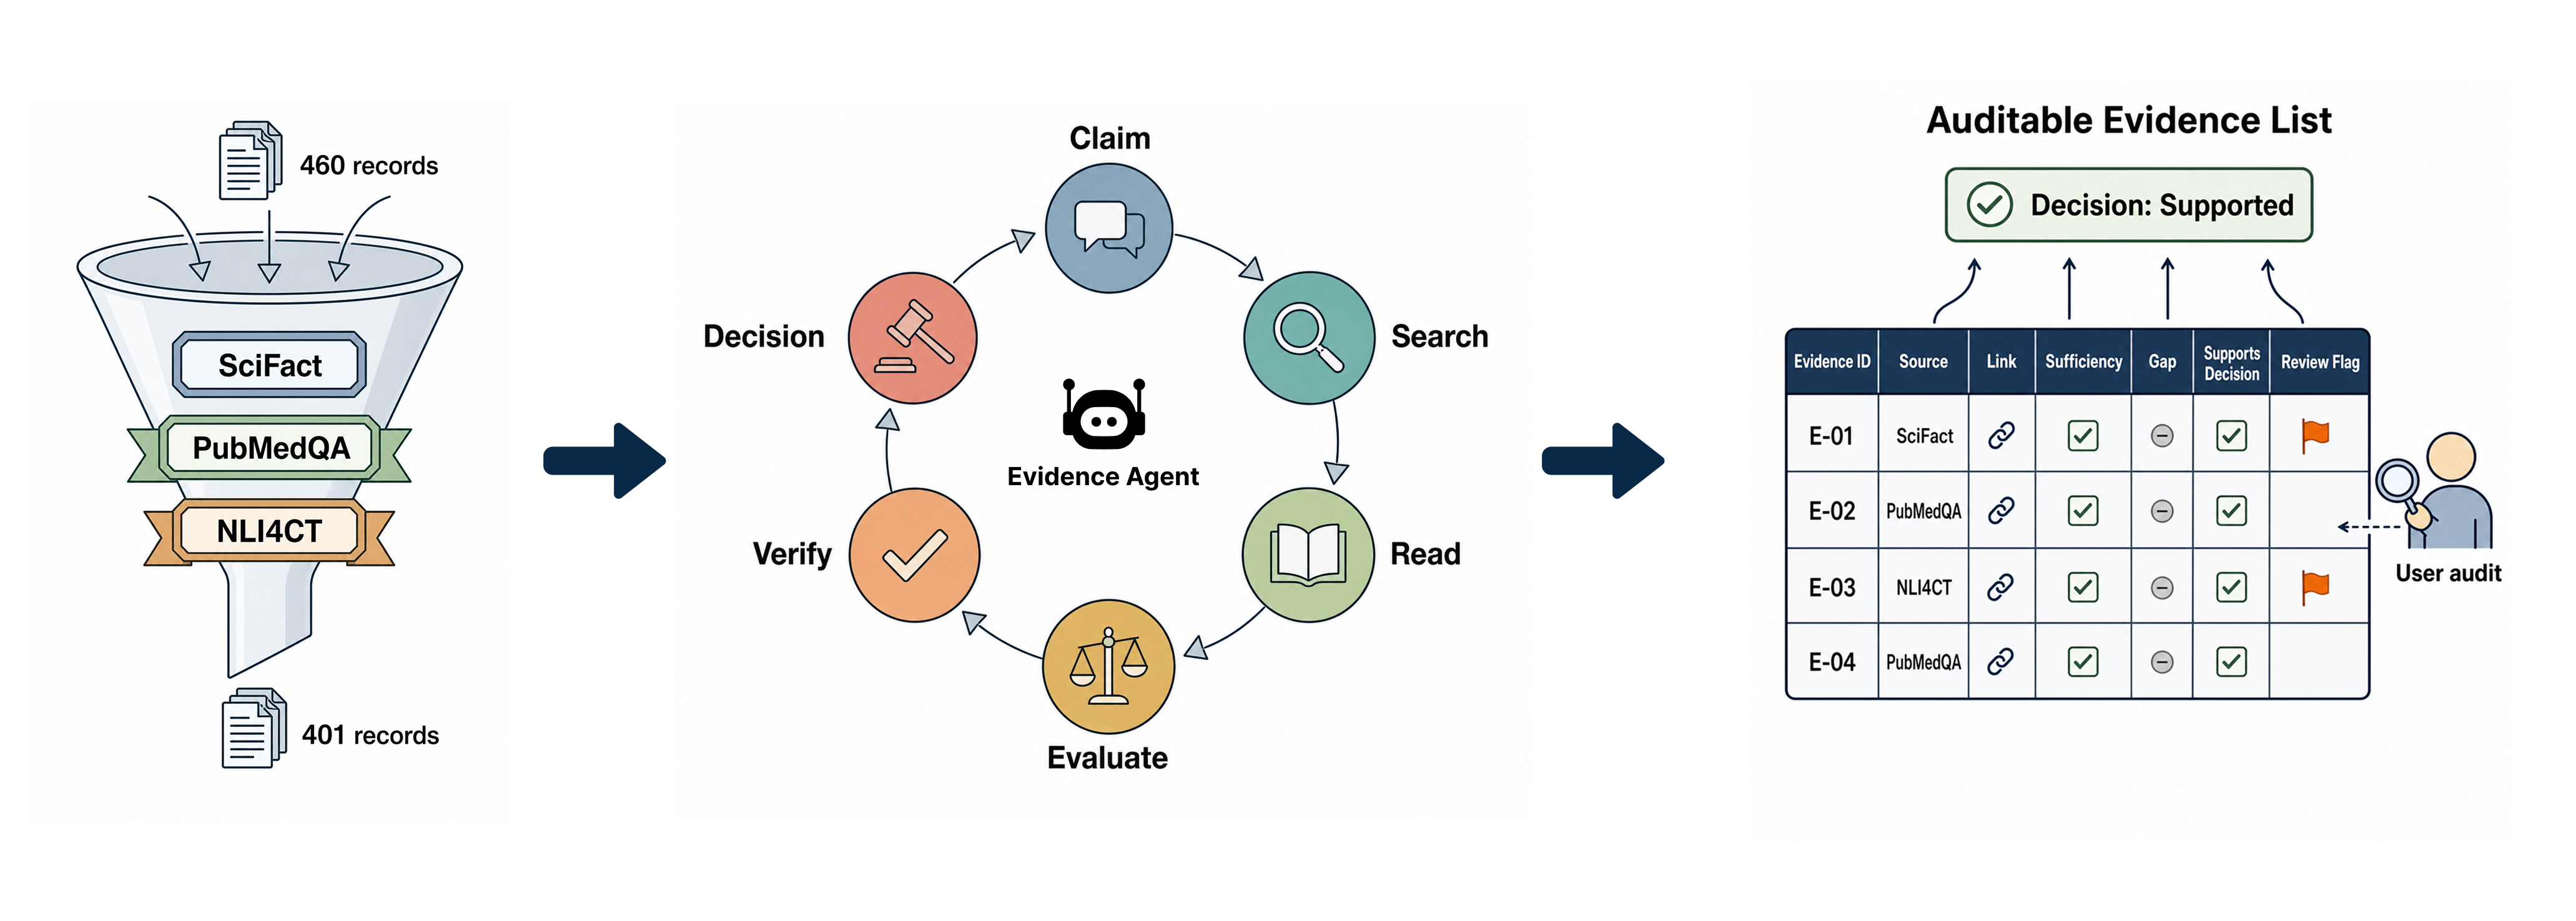
\includegraphics[width=\linewidth]{../figures/edl_main.png}
\caption{Study framework. Public-source records are audited for evaluability, converted into a unified benchmark, processed by comparison methods, and scored for decision accuracy, evidence coverage, citation validity, process validity, and automated review routing.}
\label{fig:study-framework}
\end{figure}

\section*{Statement of Significance}

\begin{center}
\small
\begin{tabular}{@{}p{0.28\linewidth}p{0.66\linewidth}@{}}
\toprule
Problem or issue & Biomedical AI systems may answer with citations without a record of evidence sufficiency, gaps, conflicts, provenance, or review needs. \\
What is already known & Evidence-based medicine, evidence-to-decision approaches, RAG, ReAct, and biomedical verification benchmarks address evidence use, retrieval, tool traces, labels, or evidence selection. \\
What this paper adds & EDL defines an evidence-based decision-loop methodology and evaluates one agent/controller implementation for benchmark-defined evidence binding, structural record validity, and review routing. \\
Who would benefit & Developers, evaluators, informatics researchers, and expert reviewers who need pre-deployment audit and failure localization. \\
\bottomrule
\end{tabular}
\end{center}

\section{Background and Related Work}

\subsection{Evidence chains and evidence-to-decision reasoning}

Evidence-based medicine describes clinical decisions as requiring explicit and judicious use of current best evidence together with clinical expertise \cite{sackett1996ebm}. Systematic-review methodology similarly treats evidence synthesis as a critical link in a chain that connects primary evidence to clinical decisions \cite{mulrow1997chain,cook1997synthesis}. These traditions motivate a basic requirement for biomedical AI evaluation: the final answer should be linked to evidence in a way that can be inspected rather than inferred from free text.

Evidence-to-decision frameworks make this separation more explicit by distinguishing the evidence base from the judgments used to reach recommendations \cite{alonso2016etd1,alonso2016etd2}. EDL does not perform guideline-grade evidence synthesis or replace expert deliberation. It operationalizes a narrower, decision-level version of the same principle: for each AI-assisted biomedical statement or question, the submitted artifact should expose the evidence state, citation basis, unresolved gaps or conflicts, and review status.

\subsection{Evidence-grounded biomedical AI}

Biomedical AI systems are increasingly evaluated in tasks that require evidence grounding rather than unconstrained text generation \cite{rajpurkar2022health,topol2019highperformance,esteva2019deep}. Scientific claim verification, biomedical question answering, and clinical-trial inference provide public-source settings with task-specific labels, documents, and evidence or context structures \cite{wadden2020scifact,jin2019pubmedqa,jullien2023nli4ct}. To support cross-source agent comparisons, we converted these source-native materials into a common record format with citable segments and scoring fields.

\subsection{RAG and tool-using agents}

Retrieval-augmented generation (RAG) links generation to retrieved evidence, and ReAct-style agents interleave reasoning and tool use \cite{lewis2020rag,yao2023react}. In this study, ReAct is treated as a tool-using, agentic RAG baseline because it searches and reads a fixed evidence library before submitting a decision. This baseline is important because it exposes tool traces and provides a strong comparison for evidence-seeking behavior. EDL differs from ReAct by requiring a structured evidence-decision record and validation contract, rather than relying on the visibility of the tool trace alone.

\subsection{Auditability and review governance}

Biomedical AI evaluation also requires attention to intended use, explainability, quality management, provenance, and human-AI interaction \cite{mcnamara2024clinicianai,overgaard2023qms,castner2024expertgaze,wekenborg2025humanai}. Provenance standards emphasize information about entities, activities, and people involved in producing a data object, which can support judgments about quality, reliability, and trustworthiness \cite{w3cprov2013}. Clinical decision-support guidance likewise emphasizes whether a health professional can independently review the basis for software recommendations \cite{fda2022cds}. EDL contributes to this line of work by operationalizing auditability at the level of the decision artifact. It asks whether the output records the evidence state in a form that can be checked by software and reviewed by humans. The method therefore complements, rather than replaces, expert review and clinical governance.

The related approaches are complementary rather than interchangeable. Table \ref{tab:edl-positioning} distinguishes the decision-level requirements that EDL makes explicit from evidence-to-decision frameworks, RAG, ReAct-style tool traces, and generic provenance models. The table is a conceptual positioning statement, not an empirical performance comparison.

\begin{table}[H]
\centering
\caption{Conceptual positioning of Evidence Decision Loops (EDL). ``Not intrinsic'' denotes capabilities not specified by the cited original formulation; they may be added in later extensions or individual implementations.}
\label{tab:edl-positioning}
\resizebox{\linewidth}{!}{%
\begin{tabular}{p{0.18\linewidth}p{0.25\linewidth}p{0.27\linewidth}p{0.22\linewidth}}
\toprule
Approach & Primary contribution & Not intrinsic to the approach & EDL distinction \\
\midrule
Evidence-to-decision frameworks \cite{alonso2016etd1,alonso2016etd2} & Separate evidence from the judgments used in recommendations & An executable, record-level protocol for LLM-supported reasoning & Requires a structured evidence-decision record and validation contract for each submitted decision \\
RAG \cite{lewis2020rag} & Conditions generation on retrieved evidence & Explicit evidence sufficiency, gap/conflict recording, or review routing & Treats retrieval or evidence receipt as one step in an auditable decision loop \\
ReAct \cite{yao2023react} & Interleaves tool use and reasoning actions & A decision-level evidence contract or validation of the submitted record & Requires cited identifiers, recorded assessments, and validation before submission \\
Provenance models \cite{w3cprov2013} & Represent entities, activities, and agents involved in data production & Source-native decision labels, evidence sufficiency, or review-routing criteria & Couples provenance with evidence assessments and decision-specific review signals \\
EDL (this study) & Defines an auditable evidence-decision protocol for biomedical AI reasoning & --- & Specifies reusable record fields, validation requirements, and review-routing triggers that are evaluated through observable artifacts \\
\bottomrule
\end{tabular}%
}
\end{table}

\section{Evidence Decision Loop Method}

\subsection{Method overview}

We define an Evidence Decision Loop as an evidence-based decision-loop methodology that takes a biomedical statement or question, an admissible evidence source, and a source-native label space as input; iteratively acquires or receives evidence; assesses evidence sufficiency; requires structured citation and gap/conflict recording; validates the submitted evidence-decision record against a validation contract; and flags records for downstream review when evidence, citation, process, or conflict criteria are not satisfied.

The present study evaluates a single-layer implementation of EDL. Each benchmark item is treated as an atomic statement or question, and evidence is represented as a flat set of source-native citable segments. The current EDL record does not model claim-to-claim dependency, evidence-graph topology, causal pathways, or recursive claim decomposition. The key output is not only a label, but an evidence-decision record that can be scored independently of hidden model reasoning. The reported endpoints evaluate benchmark-defined evidence binding and structural record validity; they do not independently adjudicate substantive evidence sufficiency, the correctness of gap or conflict assessments, or citation entailment.

EDL is therefore a methodology-level protocol, while the controller used in this study is one implementation of that protocol. Table \ref{tab:method-implementation} separates the reusable methodology elements from the concrete implementation evaluated here.

\begin{table}[H]
\centering
\caption{General EDL methodology and this study's implementation.}
\label{tab:method-implementation}
\resizebox{\linewidth}{!}{%
\begin{tabular}{p{0.18\linewidth}p{0.38\linewidth}p{0.38\linewidth}}
\toprule
Layer & General EDL methodology & This study's implementation \\
\midrule
Input & Biomedical statement or question, admissible evidence source, source-native decision space & SciFact, PubMedQA, and NLI4CT records with fixed evidence libraries \\
Evidence loop & Evidence planning, acquisition or receipt, assessment, and record curation & Single LLM controller with given-evidence or search/read evidence access; roles implemented as logical controller functions \\
Output & Evidence-decision record with citations, evidence state, gaps, conflicts, provenance, and review routing & JSONL-compatible structured records scored by the study runner \\
Validation & Scoring contract for citations, required evidence, process, and review triggers & Programmatic scorer using document/segment identifiers and trace metadata \\
Governance signal & Review routing for unresolved evidence, citation, process, or conflict issues & Automated review flags and reasons \\
\bottomrule
\end{tabular}%
}
\end{table}

\paragraph{Intended use and non-use.}
EDL is intended for pre-deployment evaluation and research-stage audits of LLM-supported biomedical evidence reasoning operating on an admissible, record-scoped evidence corpus. It produces an evidence-decision record and review-routing reasons for a qualified human reviewer, who must inspect cited segments, unresolved gaps or conflicts, citation and process-validation results, and the source-native final decision before any downstream use. EDL is not intended to diagnose, recommend treatment, rank patients, authorize clinical action, or replace expert judgment. A review flag requires human assessment; it is not itself a clinical-safety determination.

\paragraph{Functional roles within the loop.}
For conceptual clarity, EDL distinguishes three functional roles. The \textit{Planner} formulates and updates evidence requests on the basis of the current evidence-decision record. The \textit{Assessor} evaluates evidence sufficiency, gaps, conflicts, citation validity, and process requirements. The \textit{Curator} maintains the evidence-decision record, including citations, trace, provenance, validation results, and review-routing reasons. The source-native final decision remains separate from the evidence state.

In this implementation, these functions were operationalized by a controller around the model rather than as a single prompt. In the given-evidence setting, the controller received all record evidence as viewed segments. In the evidence-seeking setting, it used a fixed evidence library through search and read tools. The first search query was either produced by an optional source-aware query-planning step or, when that step was not enabled, initialized from the original statement or question. When evidence was judged insufficient, the controller requested additional evidence and updated the query using the returned next-query instruction before searching again. In source configurations that enabled the optional pre-submission citation self-check, a self-check identifying unresolved citation coverage could also request another evidence round.

After the evidence-sufficiency loop, the controller obtained a draft decision record. The optional model-mediated pre-submission citation self-check was enabled for the NLI4CT main configuration but not for the SciFact or PubMedQA main configurations. Across all sources, a deterministic programmatic post-submission validation checked structural scoring-contract requirements, including cited document and segment identifiers, recorded gap and conflict assessments, process validity, and review-routing triggers; it was distinct from the optional model-mediated self-check and did not adjudicate citation entailment or substantive evidence sufficiency. Thus, this EDL implementation was evaluated through the observable decision record and tool/process trace, not through hidden model reasoning.

\begin{algorithm}[H]
\DontPrintSemicolon
\caption{Evidence Decision Loop protocol}
\label{alg:edl-protocol}
\KwIn{decision problem $x$; admissible evidence source $S$; source-native label space $Y$; validation contract $V$; iteration budget $B$}
\KwOut{auditable evidence-decision record $R$}
Initialize $R$ with $x$, empty citations, assessments, gaps, conflicts, trace, and provenance\;
Set $z \leftarrow \textit{insufficient}$, $c \leftarrow \textsc{false}$, $b \leftarrow 0$, and $q \leftarrow \mathrm{PlanEvidenceRequest}(x)$\;
\While{$(z = \textit{insufficient} \lor \neg c) \land b < B$}{
  $E \leftarrow \mathrm{AcquireOrReceive}(S, q)$\;
  Append $(E, q)$ and access metadata to $R.\textit{trace}$ and $R.\textit{provenance}$\tcp*[r]{preserve observable evidence access}
  $(z, G, C) \leftarrow \mathrm{AssessEvidence}(x, E, R)$\;
  Record $z$, gaps $G$, and conflicts $C$ in $R$\;
  $y \leftarrow \mathrm{DraftDecision}(x, R)$ with $y \in Y$\tcp*[r]{evidence state does not determine label}
  Record $y$ and cited document--segment identifiers in $R$\;
  $c \leftarrow \mathrm{CitationsValid}(R)$\;
  \If{$(z = \textit{insufficient} \lor \neg c) \land b + 1 < B$}{
    $q \leftarrow \mathrm{UpdateEvidenceRequest}(x, R)$\;
  }
  $b \leftarrow b + 1$\;
}
$v \leftarrow \mathrm{Validate}(R, V)$\tcp*[r]{check citation and process requirements}
\If{$z \in \{\textit{insufficient}, \textit{conflicting}\} \lor \neg c \lor \neg v \lor \mathrm{RuntimeIssue}(R)$}{
  Attach review-routing reasons to $R$\tcp*[r]{route unresolved cases conservatively}
}
\KwRet{$R$}\;
\end{algorithm}

Algorithm \ref{alg:edl-protocol} expresses these logical roles procedurally: the Planner controls evidence requests, the Assessor determines the evidence state and validation results, and the Curator maintains the auditable record and review-routing reasons.

\begin{figure}[H]
\centering
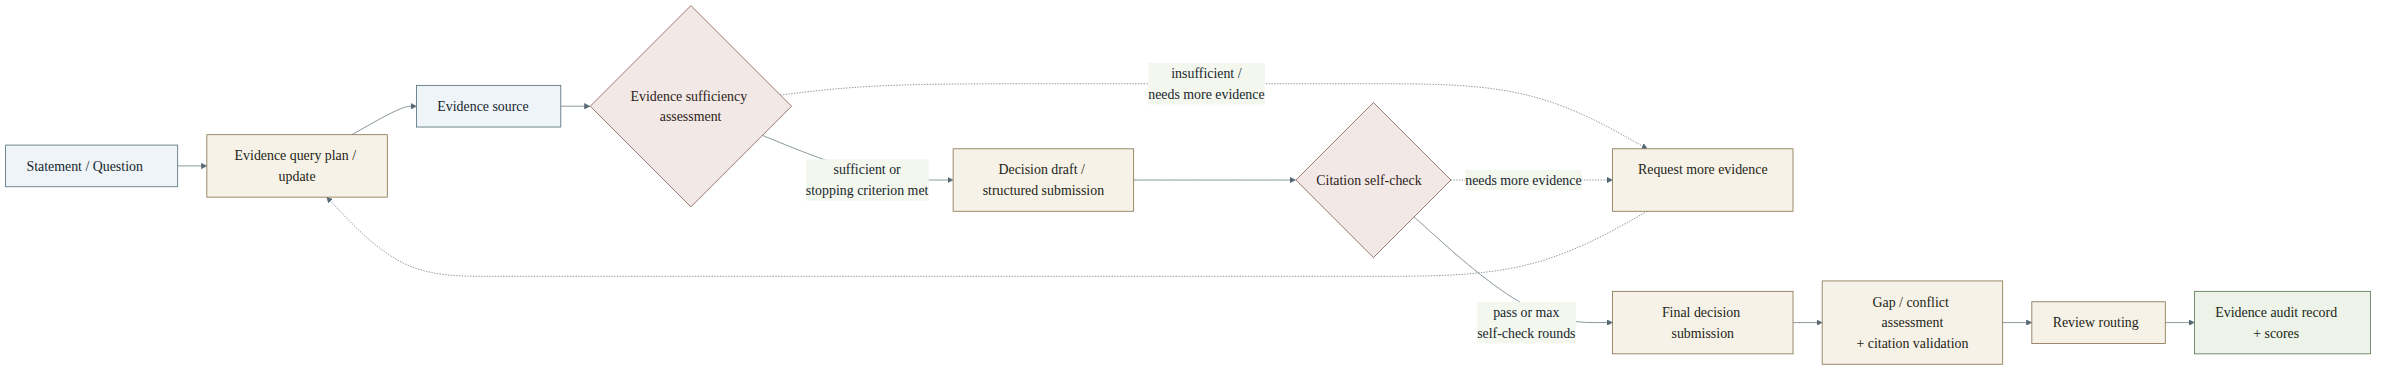
\includegraphics[width=\linewidth,keepaspectratio]{../figures/edl_workflow_english.png}
\caption{Evidence Decision Loop workflow and auditable decision-record architecture. EDL turns a decision problem and evidence-access process into a structured record containing the statement or question, cited evidence identifiers, evidence assessments, gaps, conflicts, review routing, final decision, and provenance.}
\label{fig:edl-workflow}
\end{figure}

\subsection{Decision states}

EDL separates the source-native final decision from the evidence state and review-routing status. The final decision must be one of the allowed labels for the source record. Evidence sufficiency is assessed separately as sufficient, insufficient, or conflicting, and unresolved insufficiency, material gaps or conflicts, missing or invalid citations, and runtime failures can trigger automated review routing. Conflicting evidence is therefore treated as a review-triggering evidence state even when a stopping condition requires the controller to proceed to structured submission. A plausible natural-language rationale is not sufficient if the cited evidence is missing, invalid, incomplete, or contradicted.

\subsection{Evidence-decision record}

The EDL record combines record metadata, the source-native task or claim, the final decision, cited document and segment identifiers, evidence assessments, gap and conflict assessments, review-routing flags, process trace metadata, scores, and provenance. The complete schema is provided in Supplementary Table S9. Missing or malformed structured fields are treated as missing or invalid rather than inferred from free text.

\subsection{Audit and scoring contract}

The scoring contract checks whether cited document and segment identifiers exist in the current record, whether required evidence was cited and accessed, whether the final decision matches the source label, whether the process trace contains the required search or read, assessment, and validation steps, and whether review routing was triggered for evidence insufficiency, material gaps or conflicts, citation failures, or runtime errors. This separates final-answer error, evidence-access error, citation error, process error, and review-routing error.

\begin{table}[H]
\centering
\caption{EDL components mapped to audit risks and evaluation checks.}
\label{tab:method-risk}
\resizebox{\linewidth}{!}{%
\begin{tabular}{p{0.22\linewidth}p{0.25\linewidth}p{0.27\linewidth}p{0.20\linewidth}}
\toprule
Audit risk & EDL component & Record field or trace element & Evaluation check \\
\midrule
Unsupported answer & Evidence sufficiency assessment & Evidence state; cited evidence identifiers & Required evidence recall \\
Invalid or unverifiable citation & Citation self-check and final validation & Cited document and segment identifiers & Citation validity \\
Hidden uncertainty & Gap and conflict assessment & Gap and conflict fields & Review-routing triggers \\
Opaque evidence process & Search/read trace and provenance & Process trace metadata & Process validity \\
Unsafe automation & Review routing & Review flag and review reasons & Review rate and review reasons \\
\bottomrule
\end{tabular}%
}
\end{table}

\section{Benchmark and Data Construction}

\subsection{Source-first benchmark design}

The benchmark is source first: it preserves public source labels and evidence annotations rather than synthesizing new clinical judgments. Each record includes public-source metadata, a biomedical claim or question, one or two source documents with segment-level text, required evidence identifiers, a source-native gold decision, allowed decision labels, and a JSONL structure readable by the runner and scorer.

\subsection{Main evaluation dataset}

We constructed a canonical candidate set of 460 public-source records from SciFact, PubMedQA, and NLI4CT. Before comparative execution, we performed an LLM-assisted pre-evaluation consistency audit to identify records suitable for programmatic benchmark scoring. The audit assessed whether source-native labels, allowed decision labels, required evidence identifiers, locatable evidence segments, and scoring fields were mutually consistent. It was determined from source-record audit metadata without access to outputs from Direct, CoT, ReAct, or the EDL implementation.

The audit retained 390 records for the main evaluation: 135 SciFact records, 125 PubMedQA records, and 130 NLI4CT records. The retained records contain 1413 required evidence segments and constituted the locked comparative-evaluation manifest used for every workflow. The 70 non-retained records comprised 15 SciFact, 25 PubMedQA, and 30 NLI4CT records; they were not rerun or rescored post hoc. We assigned these records to a derived, mutually exclusive exclusion-reason taxonomy based on audit outputs. Categories were applied in priority order: label-evidence disagreement, unclear label support, insufficient or partial required evidence, evidence granularity or missing-context problems, and other scoring-protocol refinement. Among the 70 non-retained records, 50 were categorized as label-evidence disagreement, 12 as unclear label support, and 8 as insufficient or partial required evidence. Source composition, exclusion-reason summaries, and the cohort-construction and execution chronology are reported in the supplement.

All three sources used the same evidence-construction workflow. Each candidate record was converted into source documents, citable segments, required \texttt{documentId}/\texttt{segmentId} evidence identifiers, source-native decisions, allowed label sets, and JSONL scoring records. Source differences were preserved in task semantics and segment granularity rather than in the scoring protocol.

\begin{figure}[H]
\centering
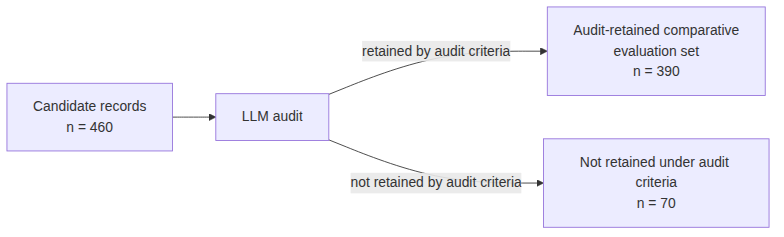
\includegraphics[width=0.92\linewidth]{../figures/dataset_audit_flow_mermaid_english.png}
\caption{Dataset construction and pre-evaluation consistency-audit flow. The 460 candidate records yielded 390 audit-retained comparative-evaluation records and 70 records not retained under the audit-defined evaluability criteria. Records were retained when source labels, required evidence identifiers, locatable segments, and programmatic scoring were mutually consistent. Retention was determined before comparative execution without access to tested-method outputs; the same locked record manifest was used for all workflows, and non-retained records were not rerun or rescored post hoc.}
\label{fig:dataset-audit-flow}
\end{figure}

Source composition of the candidate, retained, and non-retained records is provided in the supplement. The main evaluation records contained between 1 and 61 required evidence segments. Two hundred fifty records required one segment, 42 required two segments, 54 required three to five segments, and 44 required six or more segments. We used required evidence count as an operational stratification of evidence complexity, not as a complete model of open-ended clinical evidence synthesis.

\subsection{Data governance}

The benchmark uses public biomedical and clinical-trial evidence sources and avoids private patient records, credentialed clinical records, and protected health information. This design supports reproducible pre-deployment evaluation but does not establish clinical safety, diagnostic utility, or autonomous workflow readiness. The reporting package is organized around input JSONL files, trace JSONL files, result JSON files, figure source data, and reproducibility manifests.

\section{Experimental Design}

\subsection{Evaluation settings and comparison methods}

The automated experiments used two complementary settings to test one operationalization of the EDL methodology. In the given-evidence setting, relevant source segments were provided in the model context. This setting isolates evidence interpretation, citation quality, and decision-record quality. In the evidence-seeking setting, agents received the task and a searchable fixed evidence library; they had to search and read evidence before submitting a final decision.

All comparison methods used the same source-native records, allowed decision labels, citation format, and scoring contract. Direct prompted the model to produce the structured final answer in a single step. CoT used a reasoning-oriented prompt but was evaluated only on the submitted structured output rather than on hidden or free-form reasoning. ReAct used the same fixed evidence library as the EDL implementation in the evidence-seeking setting and interacted with search and read tools before submitting a structured final decision. The EDL implementation used the same evidence-access tools but added controller-level evidence-sufficiency assessment, citation validation, process validation, and derived review routing.

The primary baseline-fairness controls were therefore equality of records, source-native labels, admissible evidence libraries, search and reading tools, citation identifiers, model backend, output schema, and scoring code. ReAct was selected as the primary evidence-seeking baseline because it is a strong tool-using and agentic RAG comparator rather than an answer-only strawman. The estimand is a workflow-level contrast between ReAct-style and EDL-controlled evidence reasoning under matched evidence access and scoring, not a component-level or compute-equivalent estimate of any individual controller feature. Iterative evidence seeking, sufficiency assessment, citation validation, process validation, and derived review routing are constitutive elements of the evaluated EDL workflow. Complete run configuration, prompt artifacts, fallback handling, and trace counts are reported in the supplement; resource differences are addressed as a limitation rather than interpreted as evidence of equal-compute efficiency.

\begin{table}[H]
\centering
\caption{Comparison methods.}
\resizebox{\linewidth}{!}{%
\begin{tabular}{p{0.15\linewidth}p{0.12\linewidth}p{0.45\linewidth}p{0.22\linewidth}}
\toprule
Setting & Method & Evidence access & Role \\
\midrule
Given evidence & Direct & Relevant evidence segments supplied in context & Answer-only baseline \\
Given evidence & CoT \cite{wei2022cot} & Relevant evidence segments supplied in context & Reasoning-prompt baseline \\
Given evidence & ReAct \cite{yao2023react} & Context evidence plus tool-style trajectory & Tool-use baseline \\
Given evidence & EDL implementation & Context evidence plus structured evidence-decision record & Operationalized EDL methodology \\
Evidence seeking & ReAct \cite{yao2023react} & Fixed evidence library with BM25 search and segment reading \cite{robertson1995okapi,robertson2009bm25} & Tool-using / agentic RAG baseline \\
Evidence seeking & EDL implementation & Fixed evidence library with BM25 search, segment review, evidence assessment, and validation & Operationalized evidence-decision loop \\
\bottomrule
\end{tabular}%
}
\end{table}

\subsection{Evidence-seeking controls}

The evidence-seeking setting used BM25 retrieval to reduce differences in search space \cite{robertson1995okapi,robertson2009bm25}. For EDL, the SciFact and PubMedQA main configurations used BM25 with a controller-fixed top-5 return limit, whereas the longer NLI4CT records used source-aware query planning, BM25 neighbor expansion, and the same controller-fixed top-5 limit. ReAct could request between 1 and 10 returned segments under its tool schema and predominantly requested 5 or 10; consequently, retrieval depth and reasoning effort were workflow properties rather than equal-compute controls. ReAct used a prespecified forced-submit fallback when the configured tool budget was exhausted; the fallback allowed final decision submission but no further search or reading, and these traces were retained rather than excluded. The EDL controller added evidence-sufficiency assessment and controller-enforced citation-identifier requirements. The optional model-mediated pre-submission citation self-check was source specific, whereas the deterministic programmatic scoring-contract validation was applied after submission.

The search tool was record scoped rather than open-web retrieval. For each evidence-seeking record, \texttt{search\_segments} queried only the fixed evidence library attached to that record and returned candidate segment identifiers, snippets, and metadata. Agents then used \texttt{read\_segment} to inspect the full frozen segment text before citing it. ReAct and the EDL implementation used the same search and read tools, the same admissible citation identifiers, and the same scoring contract. This design made the evidence-seeking comparison focus on tool-use and evidence-decision behavior rather than on differences in external retrieval access.

\subsection{Main evaluation, cross-model check, and ablation analyses}

The main evaluation used \texttt{gpt-5.5}. Both settings used the same 390 main evaluation records. The given-evidence setting produced 1560 traces across Direct, CoT, ReAct, and EDL. The evidence-seeking setting produced 780 traces across ReAct and EDL. Trace-level metadata, including model and reasoning-effort fields, were retained in the reproducibility package.

We used two supplementary analyses to assess model dependence and EDL component contribution without redefining the main evaluation dataset. MiniMax-M3 was used as a cross-model check. For each source in the component analysis, the Full EDL reference was reused directly from the main evidence-seeking experiment; no additional model inference was performed for either Full reference row. The three SciFact feature-removal variants were newly executed on the same 135 records with the SciFact main configuration (\texttt{gpt-5.5}, medium reasoning effort, BM25, controller-fixed top-5 retrieval, a maximum of three evidence rounds, a minimum of two rounds and three viewed segments before sufficiency, and no citation self-check), configured to remove iterative evidence seeking, evidence-sufficiency assessment, or controller-level citation validation. The NLI4CT variants retained the NLI4CT source-specific retrieval configuration, including source-aware query planning, BM25 neighbor expansion, and fixed top-5 retrieval. Its optional citation self-check was retained except in the no-citation-validation variant. In that variant, the cited-identifier output rule and citation-error validation/repair gate were disabled, but post-submission benchmark scoring still calculated citation-identifier validity. The ablations therefore provide descriptive within-source configuration contrasts, not a pooled comparison under a uniform cross-source runtime configuration or estimates of isolated component effects.

\subsection{Blinded clinical-expert auditability evaluation}

We conducted a blinded comparative audit using 60 selected cases from SciFact and NLI4CT. Each case contributed one ReAct and one EDL report, yielding 120 report stimuli. Method identity and benchmark-derived correctness fields were concealed from clinical expert raters; reports were displayed as anonymous report formats. Eight clinical experts each assessed 60 assigned reports: 30 EDL and 30 ReAct reports. For each case, four experts assessed the ReAct report and four non-overlapping experts assessed the EDL report, so that no expert saw both formats for the same case. This design yielded four ratings per stimulus and 480 final ratings. A prespecified seed generated the balanced format allocation and a separate seeded random order for each rater's assigned reports.

\paragraph{Expert eligibility and recruitment.}
Eligible raters were licensed physicians at attending level or above, with at least five years of clinical experience and expertise in biomedical evidence appraisal, clinical research, or medical AI. Experts were purposively recruited from four specialties at Zhongshan Hospital, Fudan University. Individuals involved in EDL development, study design, case selection, report generation, or data analysis were excluded. Experts independently evaluated anonymized reports under blinded conditions. All provided written informed consent, participated voluntarily, and received no compensation.

The sample was constructed to balance preclassified output-success and output-failure patterns across source and report format. It was designed to assess the detectability of preclassified benchmark failures, rather than to estimate the prevalence of system errors or overall performance in an unselected deployment population. A preclassified benchmark failure was a report that did not jointly satisfy a correct final decision and the primary answer-and-evidence-binding metric. Raters classified each report as acceptable or requiring interception and recorded review time, confidence, and cognitive load.

Raters received standardized written instructions. They selected acceptance when the displayed evidence supported the system decision and the decision record was sufficiently clear; they selected interception when the decision appeared wrong, unsafe, contradicted by the evidence, or insufficiently supported for acceptance. Confidence was rated from 1 (very low confidence in the rater's own judgment) to 5 (very high confidence); cognitive load was rated from 1 (very easy to audit) to 5 (very difficult to audit). The complete instructions are archived in the audit bundle.

The analytic export was frozen after audit completion. It contained 485 saved submissions; for the five assignments with multiple saved revisions, we retained the highest revision number, yielding 480 final ratings. No final records were missing acceptability, confidence, cognitive-load, or elapsed-time fields. No duration-based exclusions were applied; observed review times ranged from 16.2 to 356.9 seconds, and time outcomes are reported descriptively.

\section{Metrics and Statistical Analysis}

We organized metrics by evaluation role rather than treating all outputs as co-primary endpoints. The primary evaluation metric was a joint answer-and-evidence success metric: a binary record-level score equal to 1 only when the final decision is correct, all citations are valid, and required evidence recall is 1. This composite metric was chosen because final-label accuracy alone can reward unsupported correctness, whereas evidence-supported biomedical AI also requires complete and structurally valid evidence binding.

The primary metric is an answer-and-evidence binding endpoint rather than a replacement for final-label accuracy. To assess whether conclusions depended on this strict composite definition, we also examined component endpoints and source-balanced summaries: final-label accuracy, required evidence recall, required evidence precision, citation validity, read recall in the evidence-seeking setting, and source-balanced primary metric. These sensitivity endpoints were used to interpret the direction and locus of method differences rather than as additional multiplicity-adjusted hypothesis tests.

Core secondary metrics measured final-label correctness and evidence coverage. Decision accuracy is exact agreement between the submitted decision and the source-native gold decision. Required evidence recall is the proportion of gold required evidence segments covered by valid final citations. Required evidence precision is the proportion of valid final citations that are required evidence segments.

Process diagnostic metrics characterized whether the evidence workflow produced inspectable and structurally valid artifacts. Citation validity requires every cited evidence segment to exist in the current record and to include both a valid \texttt{documentId} and \texttt{segmentId}. This is a structural identifier-validity measure; it does not by itself assess citation entailment, substantive evidence quality, or whether the evidence is sufficient for the claim. In the evidence-seeking setting, read recall measures whether segments opened through reading tools or EDL-based inspection covered required evidence. Search-output coverage is also computed from tool traces, but we treat it as a diagnostic measure for failure localization rather than as a primary comparative endpoint: the EDL implementation explicitly uses sufficiency-driven query updates, whereas ReAct uses the search tool without the same evidence-loop controller. Process validity evaluates externally recorded process steps rather than hidden model reasoning.

Governance metrics describe automated review routing produced by the EDL implementation. The review-routing rate is the proportion of records with \texttt{requiredHumanReview=true}. Review reasons include insufficient evidence, material gaps, material conflicts, missing or invalid citations, parse errors, tool errors, model errors, and forced source labels when the label space does not allow abstention. These metrics estimate review-queue size and conservatism; they do not represent completed expert review.

A tabular metric dictionary is provided in the supplement. The current analysis reports record-level means and source-stratified descriptive results. Because all methods in a setting are run on the same records, within-setting comparisons are paired at the record level. For paired method comparisons, we estimated 95\% confidence intervals using a record-level nonparametric paired bootstrap with 10,000 resamples. Each bootstrap sample resampled record identifiers with replacement and recomputed the paired mean difference between EDL and the comparator. For single-method descriptive estimates, we used a record-level nonparametric bootstrap. Confidence intervals were computed post hoc from record-level evaluation scores and did not require additional model inference. The intervals are descriptive and were not used for multiplicity-adjusted hypothesis testing.

Human-audit outcomes are reported descriptively at the rating level. Error interception was the proportion of ratings classified as interception among preclassified benchmark-failure reports; false interception was the proportion classified as interception among preclassified acceptable reports. An attempted crossed random-intercept logistic sensitivity analysis did not converge for either binary outcome; therefore, we do not report model-based odds ratios or confidence intervals. Because the audit was a selected, balanced rating-level sample, its descriptive results do not estimate population error prevalence, prospective review effectiveness, or clinical safety.

\section{Results}

The main evaluation completed all planned traces: 1560 traces in the given-evidence setting and 780 traces in the evidence-seeking setting. After the prespecified parsing and fallback handling, no final outputs were excluded because of missing outputs, provider failures, or invalid source-native decision labels. In the evidence-seeking setting, 83 ReAct traces used the prespecified forced-submit fallback and were included in scoring without post hoc exclusion.

\begin{figure}[H]
\centering
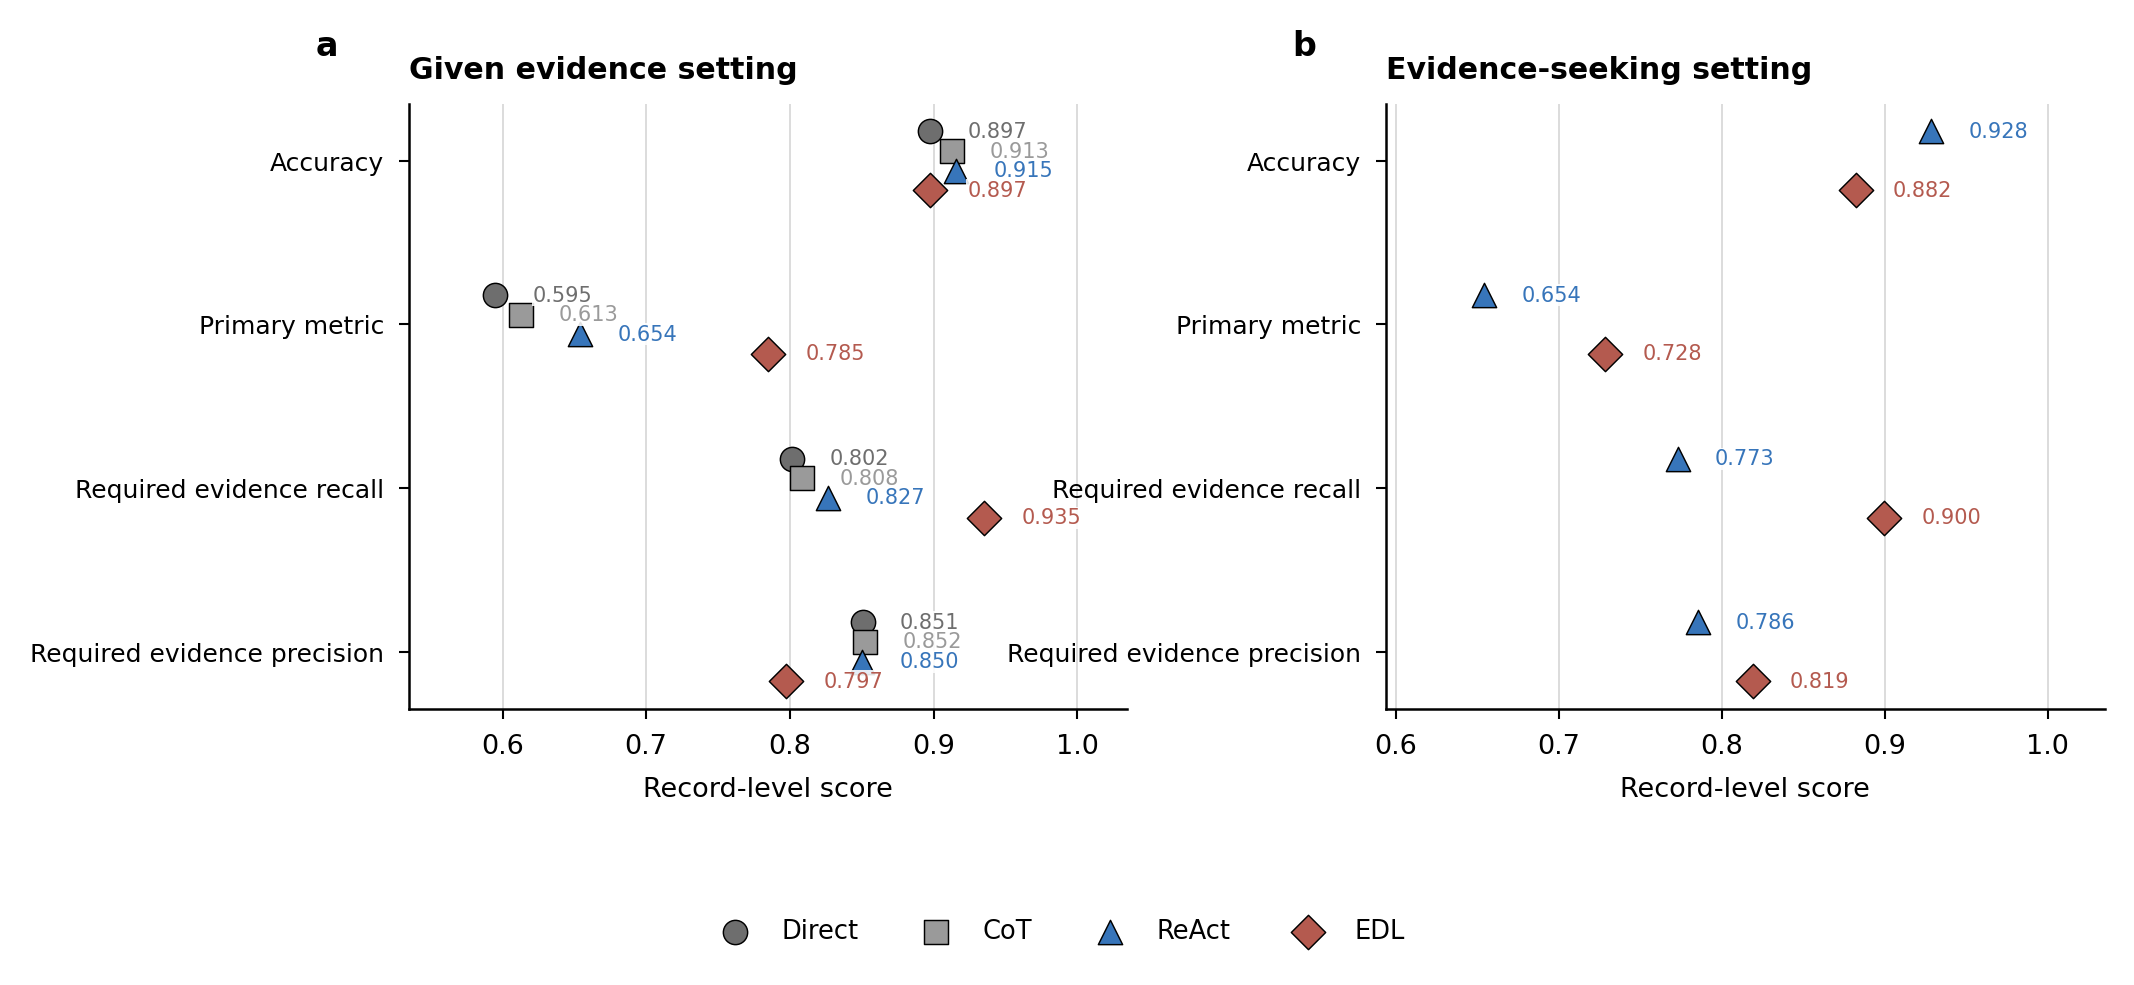
\includegraphics[width=\linewidth]{../figures/main_results_overview.png}
\caption{Primary metric overview. Points show record-level mean scores for each method. The EDL implementation improved the primary metric and required evidence recall in both settings, whereas ReAct retained the highest final decision accuracy. Paired bootstrap intervals for key evidence-seeking differences are reported in Table \ref{tab:evidence-seeking-ci}.}
\label{fig:main-results-overview}
\end{figure}

\subsection{Main results in the given-evidence setting}

In the given-evidence setting, the EDL implementation had the highest primary metric and required evidence recall, while ReAct had the highest decision accuracy. Direct and CoT remained strong when evidence was already supplied, but they did not provide an externally checkable search, reading, evidence-assessment, or validation process.

\begin{table}[H]
\centering
\caption{Main evaluation results in the given-evidence setting.}
\resizebox{\linewidth}{!}{%
\begin{tabular}{lrrrrrr}
\toprule
Method & Traces & Accuracy & Primary & Required recall & Required precision & Citation valid \\
\midrule
Direct & 390 & 0.897 & 0.595 & 0.802 & 0.851 & 0.995 \\
CoT & 390 & 0.913 & 0.613 & 0.808 & 0.852 & 0.997 \\
ReAct & 390 & 0.915 & 0.654 & 0.827 & 0.850 & 1.000 \\
EDL & 390 & 0.897 & 0.785 & 0.935 & 0.797 & 1.000 \\
\bottomrule
\end{tabular}%
}
\end{table}

This result supports the evidence coverage and audit-record advantage of the EDL implementation, but it should not be interpreted as a universal final-label accuracy advantage.

\subsection{Main results in the evidence-seeking setting}

In the evidence-seeking setting, the EDL implementation improved evidence-process metrics relative to ReAct, whereas ReAct achieved higher final decision accuracy. The EDL implementation had higher primary metric, required evidence recall, required evidence precision, read recall, citation validity, and process validity. Search-output coverage is reported as a diagnostic trace measure for localizing retrieval-stage failures, not as a primary EDL-ReAct performance endpoint.

\begin{table}[H]
\centering
\caption{Main evaluation results in the evidence-seeking setting.}
\resizebox{\linewidth}{!}{%
\begin{tabular}{lrrrrrrrr}
\toprule
Method & Traces & Accuracy & Primary & Required recall & Required precision & Read recall & Citation valid & Process valid \\
\midrule
ReAct & 390 & 0.928 & 0.654 & 0.773 & 0.786 & 0.896 & 0.997 & 0.997 \\
EDL & 390 & 0.882 & 0.728 & 0.900 & 0.819 & 0.937 & 1.000 & 1.000 \\
\bottomrule
\end{tabular}%
}
\end{table}

Table \ref{tab:evidence-seeking-ci} reports paired bootstrap confidence intervals for the main evidence-seeking comparison. The EDL implementation improved the primary metric, required evidence recall, required evidence precision, and read recall relative to ReAct. ReAct retained higher final decision accuracy.

\begin{table}[H]
\centering
\caption{Paired bootstrap confidence intervals for the evidence-seeking EDL-ReAct comparison. Differences are EDL minus ReAct.}
\label{tab:evidence-seeking-ci}
\resizebox{\linewidth}{!}{%
\begin{tabular}{lrrr}
\toprule
Metric & ReAct & EDL & Difference (95\% CI) \\
\midrule
Primary metric & 0.654 & 0.728 & 0.074 [0.026, 0.123] \\
Required evidence recall & 0.773 & 0.900 & 0.127 [0.096, 0.158] \\
Required evidence precision & 0.786 & 0.819 & 0.033 [0.006, 0.061] \\
Read recall & 0.896 & 0.937 & 0.041 [0.015, 0.068] \\
Decision accuracy & 0.928 & 0.882 & -0.046 [-0.079, -0.013] \\
\bottomrule
\end{tabular}%
}
\end{table}

Sensitivity summaries separating final-label accuracy from evidence-process endpoints showed the same pattern. ReAct retained higher final-label accuracy, whereas the EDL implementation had higher required evidence recall, required evidence precision, read recall, citation validity, and source-balanced primary metric (Supplementary Table S15).

The EDL implementation flagged 111 of 390 evidence-seeking records for review routing, a routing rate of 0.285. The most common triggers were insufficient evidence (101 records), forced source-label decisions when no abstention label was available (49 records), material gaps (10 records), and material conflicts (13 records). A single record could have multiple review reasons.

\subsection{Blinded clinical-expert auditability evaluation}

Among 120 ratings of preclassified benchmark-failure reports per method, clinical experts intercepted 73 EDL ratings (60.8\%) and 40 ReAct ratings (33.3\%). Non-interception of a preclassified benchmark failure was lower for EDL than for ReAct (39.2\% versus 66.7\%). Among 120 ratings of preclassified acceptable reports per method, false interception was lower for EDL (2/120, 1.7\%) than for ReAct (12/120, 10.0\%). Mean review time was 82.0 seconds for EDL and 99.7 seconds for ReAct; mean confidence was 3.096 and 2.908, and mean cognitive load was 2.821 and 3.650, respectively. These are descriptive rating-level results from the selected blinded audit sample; the attempted crossed random-effects sensitivity models did not converge and are not reported.

\begin{table}[H]
\centering
\caption{Blinded clinical-expert audit outcomes. Values are descriptive rating-level summaries from the selected sample.}
\label{tab:clinical-expert-audit}
\resizebox{\linewidth}{!}{%
\begin{tabular}{lrrl}
\toprule
Outcome & EDL & ReAct & Preferred direction \\
\midrule
Interception among preclassified benchmark failures & 73/120 (60.8\%) & 40/120 (33.3\%) & Higher \\
Non-interception among preclassified benchmark failures & 47/120 (39.2\%) & 80/120 (66.7\%) & Lower \\
False interception among preclassified acceptable reports & 2/120 (1.7\%) & 12/120 (10.0\%) & Lower \\
Mean review time, s & 82.0 & 99.7 & Lower \\
Mean confidence & 3.096 & 2.908 & Higher \\
Mean cognitive load & 2.821 & 3.650 & Lower \\
\bottomrule
\end{tabular}%
}
\end{table}

Preclassified failures were reports that did not jointly satisfy a correct final decision and the primary answer-and-evidence-binding metric. The balanced case-selection design does not estimate real-world error prevalence, clinical safety, or prospective workflow effects.

\subsection{Failure-mode interpretation}

The evidence-seeking failure-stage classification illustrates why audit-process metrics and final-label accuracy should be interpreted separately. In a diagnostic search-output coverage analysis, ReAct's dominant localized failure mode was retrieval miss: required evidence was not returned by search in 363 of 390 evidence-seeking traces. The EDL implementation reduced retrieval misses to 9 traces, consistent with its sufficiency-driven query-updating loop, but still had 58 citation-miss traces and 39 decision-miss-after-evidence traces, in which the evidence process was stronger than the submitted source-native label. This pattern is consistent with the main result: the EDL implementation improved evidence discovery and record auditability, whereas ReAct retained higher final decision accuracy in the all-source evidence-seeking setting.

\subsection{Source and evidence-complexity stratification}

The advantages and limitations of the EDL implementation varied by source. In SciFact, the EDL implementation achieved a higher primary metric and required evidence recall than ReAct, despite lower decision accuracy. PubMedQA was the clearest accuracy trade-off case: both methods reached complete required evidence coverage and complete read recall, but the EDL implementation had lower final \texttt{yes/no/maybe} decision accuracy and primary metric than ReAct (0.768 vs 0.912). The PubMedQA deficit was concentrated in label calibration rather than retrieval: among 29 EDL PubMedQA errors, 24 were gold \texttt{maybe} records submitted as \texttt{yes} or \texttt{no}, and five were gold \texttt{yes/no} records submitted as \texttt{maybe} (Supplementary Table S16). This pattern supports the distinction between benchmark-defined evidence binding and final-label accuracy. In NLI4CT, the EDL implementation substantially improved read recall, required evidence recall, and primary metric relative to ReAct, but both methods were challenged by long trial reports with multiple required evidence segments.

\begin{table}[H]
\centering
\caption{Evidence-seeking source-stratified results.}
\resizebox{\linewidth}{!}{%
\begin{tabular}{llrrrrr}
\toprule
Source & Method & Traces & Accuracy & Primary & Required recall & Read recall \\
\midrule
SciFact & ReAct & 135 & 0.993 & 0.859 & 0.874 & 0.985 \\
SciFact & EDL & 135 & 0.948 & 0.874 & 0.933 & 0.967 \\
PubMedQA & ReAct & 125 & 0.912 & 0.912 & 1.000 & 1.000 \\
PubMedQA & EDL & 125 & 0.768 & 0.768 & 1.000 & 1.000 \\
NLI4CT & ReAct & 130 & 0.877 & 0.192 & 0.449 & 0.703 \\
NLI4CT & EDL & 130 & 0.923 & 0.538 & 0.768 & 0.844 \\
\bottomrule
\end{tabular}%
}
\end{table}

\begin{figure}[H]
\centering
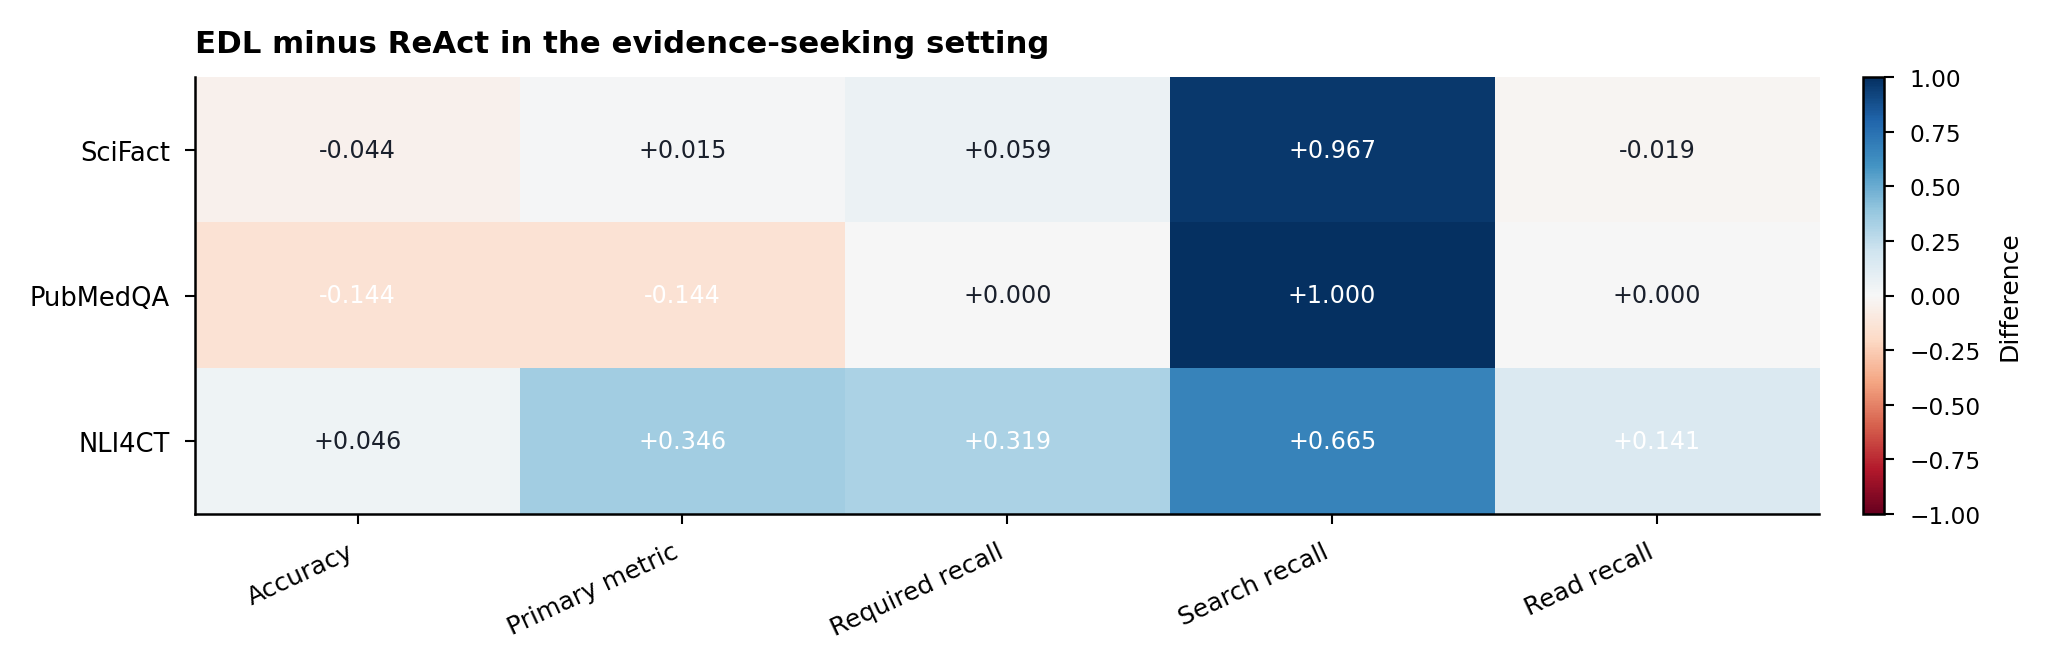
\includegraphics[width=\linewidth]{../figures/source_stratified_heatmap.png}
\caption{Source-stratified differences in the evidence-seeking setting. Cells show EDL minus ReAct record-level mean scores. Positive values favor EDL and negative values favor ReAct. Search-output coverage cells, if shown, should be interpreted as diagnostic trace measures rather than standalone retrieval benchmarks; PubMedQA showed lower final decision accuracy and primary metric for EDL.}
\label{fig:source-stratified-heatmap}
\end{figure}

Stratifying records by required evidence count showed that high-segment records were more difficult for both methods. In the given-evidence setting, EDL required evidence recall was 0.964 for one-segment records, 0.964 for two-segment records, 0.941 for three- to five-segment records, and 0.735 for records with six or more required evidence segments. In the evidence-seeking setting, the corresponding EDL recalls were 0.972, 0.917, 0.848, and 0.535. The complete matrices are provided in the supplement.

\subsection{Supplementary model and component checks}

In the SciFact evidence-seeking subset, EDL's primary metric was higher than ReAct's in both \texttt{gpt-5.5} and MiniMax-M3. With \texttt{gpt-5.5}, EDL and ReAct had primary metrics of 0.874 and 0.859, respectively. With MiniMax-M3, EDL and ReAct had primary metrics of 0.830 and 0.800, respectively. The complete SciFact cross-model and three-source MiniMax-M3 supplementary evaluations are provided in Supplementary Tables S6 and S17.

Exploratory within-source single-run configuration contrasts showed different structural-record profiles when controller components were removed; they do not estimate isolated component effects. In SciFact, removing iterative seeking reduced the primary metric from 0.874 to 0.785. Removing sufficiency assessment yielded a primary metric of 0.815 but reduced review routing from 0.385 to 0.015. Disabling controller-level citation validation reduced citation-identifier validity from 1.000 to 0.067 and the primary metric to 0.059. In NLI4CT, removing iterative seeking reduced the primary metric from 0.538 to 0.423; removing sufficiency assessment increased it to 0.577 but eliminated review routing; and disabling controller-level citation validation reduced citation-identifier validity to 0.200 and the primary metric to 0.115. The complete ablation matrix is reported in Supplementary Table S18.

\section{Discussion}

This study introduced EDL as an evidence-based decision-loop methodology and evaluated one EDL-based agent/controller implementation in public biomedical benchmark tasks. The main finding is not that EDL universally improves final-label accuracy. In the evidence-access- and scoring-matched comparison with ReAct, the evaluated implementation improved benchmark-defined evidence binding, required-evidence recall, and read recall, while yielding lower overall final-label accuracy and source-specific trade-offs. Direct and CoT can perform well when evidence is supplied, and ReAct remains a strong tool-using, agentic RAG baseline.

The informatics contribution lies in the methodology and its observable decision artifact. EDL specifies how evidence-supported AI-assisted reasoning should be structured if it is to be auditable: the source-native task or claim, cited evidence identifiers, evidence assessments, gap status, conflict status, review-routing signals, and provenance should be recorded before a final conclusion is submitted. This record can be generated by different implementations and scored independently of hidden chain-of-thought reasoning.

The supplementary analyses are consistent with this interpretation but should not be read as independent validation of deployment readiness. The MiniMax-M3 check suggests that the benchmark-defined evidence-binding pattern is not limited to the primary model backend, and the exploratory within-source component ablations suggest that the evaluated implementation depends on coordinated controller features rather than on a single prompt change. In particular, iterative evidence seeking, recorded sufficiency assessment, and citation-identifier validation affected different parts of the structural record profile; the single-run ablations do not identify isolated causal effects or equal-compute performance.

Review routing further illustrates the distinction between benchmark workflow behavior and expert adjudication. The EDL implementation flagged 111 of 390 evidence-seeking records for review routing. This estimate describes the route-to-review burden within the audit-evaluable benchmark and supports failure localization; it is distinct from completed expert review. In the selected balanced rating-level audit, EDL reports meeting the preclassified benchmark-failure definition were more often classified as requiring interception, and preclassified acceptable EDL reports were less often falsely intercepted. This conditional finding does not establish prospective reviewer effectiveness or workflow benefit.

The comparison with ReAct and RAG should therefore be framed carefully. ReAct is not a weak or irrelevant baseline; it is the relevant tool-using baseline in this study and achieved higher final decision accuracy in the all-source evidence-seeking setting. The evaluated EDL implementation should be interpreted as improving benchmark-defined evidence binding and structural record validity rather than as a general-purpose accuracy optimizer. Its citation-validity and process-validity endpoints were near ceiling for both workflows and do not establish citation entailment or substantive evidence sufficiency.

The source-stratified results show why this distinction matters. In SciFact, the EDL implementation improved the primary metric and required evidence recall. In PubMedQA, it found the required evidence but had difficulty calibrating final \texttt{yes/no/maybe} labels. This failure case shows that evidence availability and evidence binding do not by themselves solve source-native answer calibration; review routing should therefore be interpreted as a governance and failure-localization signal rather than as a substitute for label accuracy. In NLI4CT, it improved search and reading coverage in long trial reports, while both methods struggled with complete citation coverage across many required evidence segments.

The present study evaluates a single-layer implementation of EDL, but the methodology points to a natural multi-layer extension. Future work should decompose higher-level decisions into auditable claims, run extraction and evidence loops for each claim, and assemble an evidence graph that records support, contradiction, gaps, provenance, and review status. This extension can draw on clinical reasoning distinctions between data-driven forward reasoning and hypothesis-driven backward reasoning \cite{patel1986medicalreasoning,elstein1978medicalproblem}, as well as argumentation models that separate claims, evidence, warrants, rebuttals, and conflict relations \cite{toulmin1958argument,dung1995argumentation}. In this sense, a future forward evidence loop would move from observations or evidence toward claims and conclusions, whereas a backward evidence loop would move from a candidate decision, diagnosis, hypothesis, or claim toward the evidence needed to support, refute, or distinguish it. This future direction was not implemented or evaluated in the current study.

EDL is an evidence-based decision-loop methodology, and this study evaluates one pre-deployment implementation of that methodology. The present results provide initial evidence that the proposed protocol can be operationalized to produce inspectable information artifacts. They do not establish clinical safety, diagnostic efficacy, treatment utility, prospective review effectiveness, or readiness for autonomous deployment.

\section{Limitations}

First, the main evaluation used \texttt{gpt-5.5} as the primary model backend. MiniMax-M3 was included as a supplementary evaluation, but the results do not establish implementation independence across all model families, vendors, reasoning budgets, or tool-runtime configurations.

Second, the benchmark uses public biomedical and clinical-trial evidence resources rather than patient-level clinical records. This supports reproducibility and avoids protected health information, but it limits claims about deployment in clinical environments.

Third, the benchmark was restricted to records satisfying audit-defined evaluability criteria for source-label and evidence consistency. The findings therefore characterize comparative performance within this audit-evaluable benchmark population and do not establish performance for all candidate records, routine clinical care, or records outside the present audit framework. The 70 non-retained records were not rerun or rescored post hoc; their disposition is reported descriptively. They remain important targets for future adjudication.

Fourth, the evidence-seeking environment used a fixed evidence library and constrained retrieval tools. This design supports controlled comparison, but it does not represent open-web evidence gathering or all possible retrieval strategies.

Fifth, the statistical analysis remains descriptive. Record-level bootstrap intervals quantify uncertainty for the main paired automated comparisons, but they are not multiplicity-adjusted hypothesis tests and do not model all sources of variation, including prompt, model, retrieval configuration, or human-rater variation in the separate audit.

Sixth, the blinded clinical-expert audit included only 60 selected SciFact and NLI4CT cases and was balanced by preclassified output-success and output-failure patterns. It therefore does not estimate the prevalence of system failures, overall report acceptance, clinical safety, prospective reviewer effectiveness, or performance in unselected deployments. Its 480 ratings were clustered within eight raters and 120 stimuli. The attempted crossed random-effects models did not converge and are not reported; descriptive rating-level differences cannot remove the limitations of selective sampling or substitute for a larger prospective study. Method identity was concealed, although differences in report structure may have allowed some raters to infer the generating workflow. Expert review of deidentified public benchmark reports is also not equivalent to patient care, diagnostic efficacy, or clinical outcome evaluation.

Seventh, the workflows were matched for records, evidence access, and scoring, but not for reasoning-effort configuration, total model calls, tool calls, latency, token use, or monetary cost. The study therefore estimates workflow-level effectiveness rather than equal-compute efficiency.

Eighth, the main analysis used one completed output per method-record pair. The reported intervals capture variation across records rather than within-record stochasticity from repeated model executions, prompts, retrieval configurations, or provider updates. The component analysis likewise used one completed output per record and variant; its Full reference rows were reused from the earlier main experiment, whereas the SciFact feature-removal variants were executed later. Temporal or stochastic model-service drift was therefore not estimated, and the source-specific SciFact and NLI4CT configurations preclude treating the combined ablation matrix as a uniform cross-source experiment. In addition, representation of the public benchmarks in closed-model pretraining cannot be excluded.

\section{Conclusion}

Within an audit-evaluable public-source benchmark corpus, the evaluated EDL agent/controller implementation improved benchmark-defined evidence binding, required-evidence recall, and read recall relative to ReAct in the evidence-seeking setting, while ReAct retained higher overall final-label accuracy and PubMedQA showed an important EDL accuracy trade-off. Descriptively, in a separate selected blinded clinical-expert rating sample, 73/120 EDL ratings and 40/120 ReAct ratings intercepted reports meeting a preclassified benchmark-failure definition; 2/120 EDL ratings and 12/120 ReAct ratings intercepted preclassified acceptable reports. The implementation also produced review-routing flags within this benchmark. These findings provide initial evidence that the proposed EDL protocol can be operationalized to generate structurally inspectable evidence-decision records; substantive evidence sufficiency, gap/conflict correctness, citation entailment, clinical safety, and prospective human-review benefit were not established.

\section*{Data and Code Availability}

The data, code, and materials supporting the reported analyses are available in the public Evidence Decision Loops release \href{https://github.com/xiaoxubeii/evidence-decision-loops/releases/tag/v0.2.8}{\texttt{v0.2.8}} \cite{eviagent2026artifacts,eviagent2026software}; this release, rather than the mutable repository head, is the reproducibility target for this manuscript. Its release assets include the final manuscript source package and \texttt{SHA256SUMS-v0.2.8.txt}; the tagged repository contains the canonical benchmark dataset, pre-evaluation consistency-audit outputs, trace files, result summaries, bootstrap confidence-interval artifacts, figure source data, audit summaries, \texttt{gpt-5.5} dual-setting results, MiniMax-M3 supplementary results, the final S18 EDL component-ablation summary and underlying traces, prompt templates, schema files, reproducibility manifests, the EDL runner, the V4 comparison runner, the consistency-audit runner, analysis scripts, and manuscript verification utilities. The public release includes the expert-audit protocol, assignments, and anonymized report stimuli. It does not distribute completed expert-response records, access credentials, or direct identifiers. Deidentified rating data and the corresponding audit-analysis outputs are held under controlled access because they concern human participants. Requests may be directed to the corresponding author through the submission contact and are assessed under the ethics determination and institutional data-governance requirements. Materials that cannot be redistributed are identified in the repository manifest.

\section*{Ethics Statement}

This study did not involve patients, patient records, biological specimens, clinical interventions, or protected health information. The clinical-expert evaluation involved eight experts who assessed anonymized AI-generated report stimuli. The evaluation was reviewed by the Ethics Committee of Zhongshan Hospital, Fudan University and was determined to be exempt from full ethics review as minimal-risk research involving professional evaluation of anonymized materials (reference ZS09437881; June 2026). All experts provided written informed consent before participation. Participation was voluntary, and experts received no compensation. Only deidentified rating data were used for analysis and publication.

\section*{Declaration of Competing Interest}

The authors declare that they have no known competing financial interests or personal relationships that could have appeared to influence the work reported in this paper.

\section*{Funding}

This research did not receive any specific grant from funding agencies in the public, commercial, or not-for-profit sectors.

\section*{Author Contributions}

Cong Wang: Conceptualization, Methodology (clinical and experimental design), Investigation, clinical interpretation, Validation, Writing -- original draft, Writing -- review and editing. Bei Xu: Methodology (algorithm design), Software (implementation and engineering), Data curation, Formal analysis, Investigation (experiment execution), Visualization, Validation, Writing -- review and editing. All authors reviewed and approved the final manuscript.

\section*{Declaration of Generative AI and AI-Assisted Technologies in the Writing Process}

During the preparation of this work, the authors used OpenAI ChatGPT/Codex to assist with manuscript restructuring, language editing, consistency checking, and LaTeX drafting support. The authors reviewed, edited, and verified the content as needed and take full responsibility for the content of the publication. Generative AI tools were not listed as authors and were not used to make independent scientific, clinical, or statistical judgments.

\begin{thebibliography}{99}

\bibitem{sackett1996ebm}
D.L. Sackett, W.M.C. Rosenberg, J.A.M. Gray, R.B. Haynes, W.S. Richardson, Evidence based medicine: what it is and what it isn't, \emph{BMJ} 312 (1996) 71--72. \url{https://doi.org/10.1136/bmj.312.7023.71}

\bibitem{mulrow1997chain}
C.D. Mulrow, D.J. Cook, F. Davidoff, Systematic reviews: critical links in the great chain of evidence, \emph{Ann. Intern. Med.} 126 (1997) 389--391. \url{https://doi.org/10.7326/0003-4819-126-5-199703010-00008}

\bibitem{cook1997synthesis}
D.J. Cook, C.D. Mulrow, R.B. Haynes, Systematic reviews: synthesis of best evidence for clinical decisions, \emph{Ann. Intern. Med.} 126 (1997) 376--380. \url{https://doi.org/10.7326/0003-4819-126-5-199703010-00006}

\bibitem{alonso2016etd1}
P. Alonso-Coello, H.J. Schunemann, J. Moberg, R. Brignardello-Petersen, E.A. Akl, M. Davoli, et al., GRADE Evidence to Decision (EtD) frameworks: a systematic and transparent approach to making well informed healthcare choices. 1: Introduction, \emph{BMJ} 353 (2016) i2016. \url{https://doi.org/10.1136/bmj.i2016}

\bibitem{alonso2016etd2}
P. Alonso-Coello, A.D. Oxman, J. Moberg, R. Brignardello-Petersen, E.A. Akl, M. Davoli, et al., GRADE Evidence to Decision (EtD) frameworks: a systematic and transparent approach to making well informed healthcare choices. 2: Clinical practice guidelines, \emph{BMJ} 353 (2016) i2089. \url{https://doi.org/10.1136/bmj.i2089}

\bibitem{w3cprov2013}
P. Groth, L. Moreau (Eds.), PROV-Overview: an overview of the PROV family of documents, W3C Working Group Note, 30 April 2013. Available from: \url{https://www.w3.org/TR/prov-overview/}

\bibitem{fda2022cds}
U.S. Food and Drug Administration, \emph{Clinical Decision Support Software: Guidance for Industry and Food and Drug Administration Staff}, 2022. Available from: \url{https://www.fda.gov/regulatory-information/search-fda-guidance-documents/clinical-decision-support-software} (accessed 16 July 2026).

\bibitem{patel1986medicalreasoning}
V.L. Patel, G.J. Groen, Knowledge based solution strategies in medical reasoning, \emph{Cogn. Sci.} 10 (1986) 91--116. \url{https://doi.org/10.1207/s15516709cog1001_4}

\bibitem{elstein1978medicalproblem}
A.S. Elstein, L.S. Shulman, S.A. Sprafka, \emph{Medical Problem Solving: An Analysis of Clinical Reasoning}, Harvard University Press, Cambridge, MA, 1978.

\bibitem{toulmin1958argument}
S.E. Toulmin, \emph{The Uses of Argument}, Cambridge University Press, Cambridge, 1958.

\bibitem{dung1995argumentation}
P.M. Dung, On the acceptability of arguments and its fundamental role in nonmonotonic reasoning, logic programming and n-person games, \emph{Artif. Intell.} 77 (1995) 321--357. \url{https://doi.org/10.1016/0004-3702(94)00041-X}

\bibitem{moor2023foundation}
M. Moor, O. Banerjee, Z.S.H. Abad, et al., Foundation models for generalist medical artificial intelligence, \emph{Nature} 616 (2023) 259--265. \url{https://doi.org/10.1038/s41586-023-05881-4}

\bibitem{singhal2023clinical}
K. Singhal, S. Azizi, T. Tu, et al., Large language models encode clinical knowledge, \emph{Nature} 620 (2023) 172--180. \url{https://doi.org/10.1038/s41586-023-06291-2}

\bibitem{rajpurkar2022health}
P. Rajpurkar, E. Chen, O. Banerjee, E.J. Topol, AI in health and medicine, \emph{Nat. Med.} 28 (2022) 31--38. \url{https://doi.org/10.1038/s41591-021-01614-0}

\bibitem{topol2019highperformance}
E.J. Topol, High-performance medicine: the convergence of human and artificial intelligence, \emph{Nat. Med.} 25 (2019) 44--56. \url{https://doi.org/10.1038/s41591-018-0300-7}

\bibitem{esteva2019deep}
A. Esteva, A. Robicquet, B. Ramsundar, et al., A guide to deep learning in healthcare, \emph{Nat. Med.} 25 (2019) 24--29. \url{https://doi.org/10.1038/s41591-018-0316-z}

\bibitem{mcnamara2024clinicianai}
S.L. McNamara, P.H. Yi, W. Lotter, The clinician-AI interface: intended use and explainability in FDA-cleared AI devices for medical image interpretation, \emph{npj Digit. Med.} 7 (2024) 80. \url{https://doi.org/10.1038/s41746-024-01080-1}

\bibitem{overgaard2023qms}
S.M. Overgaard, M.G. Graham, T. Brereton, et al., Implementing quality management systems to close the AI translation gap and facilitate safe, ethical, and effective health AI solutions, \emph{npj Digit. Med.} 6 (2023) 218. \url{https://doi.org/10.1038/s41746-023-00968-8}

\bibitem{lewis2020rag}
P. Lewis, E. Perez, A. Piktus, et al., Retrieval-augmented generation for knowledge-intensive NLP tasks, in: \emph{Advances in Neural Information Processing Systems 33}, 2020, pp. 9459--9474. Available from: \url{https://proceedings.neurips.cc/paper/2020/hash/6b493230205f780e1bc26945df7481e5-Abstract.html}

\bibitem{yao2023react}
S. Yao, J. Zhao, D. Yu, N. Du, I. Shafran, K. Narasimhan, Y. Cao, ReAct: synergizing reasoning and acting in language models, in: \emph{Proceedings of the International Conference on Learning Representations}, 2023. Available from: \url{https://openreview.net/forum?id=WE_vluYUL-X}

\bibitem{wadden2020scifact}
D. Wadden, S. Lin, K. Lo, L.L. Wang, M. van Zuylen, A. Cohan, H. Hajishirzi, Fact or fiction: verifying scientific claims, in: \emph{Proceedings of the 2020 Conference on Empirical Methods in Natural Language Processing}, 2020, pp. 7534--7550. \url{https://doi.org/10.18653/v1/2020.emnlp-main.609}

\bibitem{jin2019pubmedqa}
Q. Jin, B. Dhingra, Z. Liu, W.W. Cohen, X. Lu, PubMedQA: a dataset for biomedical research question answering, in: \emph{Proceedings of the 2019 Conference on Empirical Methods in Natural Language Processing and the 9th International Joint Conference on Natural Language Processing}, 2019, pp. 2567--2577. \url{https://doi.org/10.18653/v1/D19-1259}

\bibitem{jullien2023nli4ct}
M. Jullien, M. Valentino, H. Frost, P. O'Regan, D. Landers, A. Freitas, NLI4CT: multi-evidence natural language inference for clinical trial reports, in: \emph{Proceedings of the 2023 Conference on Empirical Methods in Natural Language Processing}, 2023, pp. 16745--16764. \url{https://doi.org/10.18653/v1/2023.emnlp-main.1041}

\bibitem{castner2024expertgaze}
N. Castner, L. Arsiwala-Scheppach, S. Mertens, et al., Expert gaze as a usability indicator of medical AI decision support systems: a preliminary study, \emph{npj Digit. Med.} 7 (2024) 199. \url{https://doi.org/10.1038/s41746-024-01192-8}

\bibitem{wekenborg2025humanai}
M.K. Wekenborg, S. Gilbert, J.N. Kather, Examining human-AI interaction in real-world healthcare beyond the laboratory, \emph{npj Digit. Med.} 8 (2025) 169. \url{https://doi.org/10.1038/s41746-025-01559-5}

\bibitem{wilkinson2016fair}
M.D. Wilkinson, M. Dumontier, I.J.J. Aalbersberg, et al., The FAIR Guiding Principles for scientific data management and stewardship, \emph{Sci. Data} 3 (2016) 160018. \url{https://doi.org/10.1038/sdata.2016.18}

\bibitem{huerta2023fairai}
E.A. Huerta, B. Blaiszik, L. Brinson, et al., FAIR for AI: an interdisciplinary and international community building perspective, \emph{Sci. Data} 10 (2023) 487. \url{https://doi.org/10.1038/s41597-023-02298-6}

\bibitem{wei2022cot}
J. Wei, X. Wang, D. Schuurmans, et al., Chain-of-thought prompting elicits reasoning in large language models, in: \emph{Advances in Neural Information Processing Systems 35}, 2022, pp. 24824--24837. Available from: \url{https://proceedings.neurips.cc/paper_files/paper/2022/hash/9d5609613524ecf4f15af0f7b31abca4-Abstract-Conference.html}

\bibitem{robertson1995okapi}
S.E. Robertson, S. Walker, S. Jones, M.M. Hancock-Beaulieu, M. Gatford, Okapi at TREC-3, in: D.K. Harman (Ed.), \emph{Overview of the Third Text REtrieval Conference (TREC-3)}, NIST Special Publication 500-225, 1995, pp. 109--126. Available from: \url{https://trec.nist.gov/pubs/trec3/t3_proceedings.html}

\bibitem{robertson2009bm25}
S. Robertson, H. Zaragoza, The probabilistic relevance framework: BM25 and beyond, \emph{Found. Trends Inf. Retr.} 3 (2009) 333--389. \url{https://doi.org/10.1561/1500000019}

\bibitem{eviagent2026artifacts}
[dataset] C. Wang, B. Xu, Evidence Decision Loops benchmark and reproducibility artifacts [dataset], GitHub release v0.2.8, 2026. Available from: \url{https://github.com/xiaoxubeii/evidence-decision-loops/releases/tag/v0.2.8}.

\bibitem{eviagent2026software}
C. Wang, B. Xu, Evidence Decision Loops reference implementation and evaluation code [software], GitHub release v0.2.8, 2026. Available from: \url{https://github.com/xiaoxubeii/evidence-decision-loops/releases/tag/v0.2.8}.

\end{thebibliography}

\end{document}
